\subsection{Картографические проекции}

\subsubsection{Цилиндрическая равнопромежуточная проекция}

\term{Цилиндрическая равнопромежуточная проекция}, иначе плоская прямоугольная проекция, является наиболее простой проекцией сферы на плоскость. При данной проекции искажаются как углы, так и площади, \lookPicRef{pic:map-projection-plate-carree}. Неизменным остается только масштаб вдоль меридианов и экватора. 

Пусть базисная точка для построения проекции имеет географические координаты $(\lambda_0, \varphi_0)$, тогда цилиндрическая равнопромежуточная проекция определяется правилом
\begin{equation}
    \left\{\begin{aligned}
        x &= \lambda - \lambda_0,\\
        y &= \varphi - \varphi_0.
    \end{aligned}\right.
\end{equation}

\subsubsection{Цилиндрическая проекция Ламберта}

\term{Цилиндрическая проекция Ламберта} (\picRef{pic:map-projection-lambertcylindrical}) относится к семейству цилиндрических \imp{равновеликих} проекций. Задается преобразованием
\begin{equation*}
    \left\{\begin{aligned}
        x &= \lambda - \lambda_0,\\
        y &= \sin \varphi.
    \end{aligned}\right.
\end{equation*}

Докажем \term{равновеликость} данной проекции, то есть, что она переводит элементарные площадки площади $dS$ в элементарные площадки такой же площади. Для этого рассмотрим элементарную площадку с центром в точке $(\lambda, \varphi)$ на единичной сфере. Её площадь $dS_\text{сф} = \cos \varphi \, d\varphi \, d\lambda $. Теперь найдём выражение для площади её проекции~--- элементарной площадки с центром в точке $(x, y)$: 
\begin{equation*}
    dS_\text{пр} = dx \, dy = d\lambda \, d(\sin \varphi) = \cos\varphi \, d\varphi \, d\lambda = dS_\text{сф}.
\end{equation*} 
Полученное равенство завершает доказательство равновеликости цилиндрической проекции Ламберта.

\subsubsection{Проекция Меркатора}

\term{Проекция Меркатора} является конформной\footnote{равноугольная~--- сохраняющая углы} цилиндрической проекцией, \lookPicRef{pic:map-projection-mercator}. Из циндричности проекции следует, связь $x = \lambda - \lambda_0$. Получим выражение для ординаты проекции из свойства равноугольности~--- сохранения отношения масштабов по осям, которое можно записать как
\begin{equation}
    \frac{dx}{dy} = \frac{\cos \varphi \, d\lambda}{d \varphi}.
\end{equation}
Откуда, используя $dx = d \lambda$ и полагая константу интегрирования равной нулю, имеем следующее\footnote{$\lam x$~--- ламбертиан $x$}:
\begin{multline*}
    y 
        = \int dy 
%        = \int \sec \varphi \, d\varphi
        = \int \frac{d\varphi}{\cos \varphi }
        = \int \frac{\cos \varphi \,d\varphi }{\cos^2 \varphi}
        = \int \frac{\cos \varphi \, d\varphi }{1 - \sin^2 \varphi} \overset{t = \sin \varphi}{=} \\
        = \int \frac{dt}{1 - t^2} 
        = \int\frac{dt}{(1-t)(1+t)}
        = \frac{1}{2} \left( \int \frac{1}{1+t} \, dt \, + \! \int \frac{1}{1-t} \, dt \right) = \\
%        = \frac{1}{2} \ln \left|1 + t\right| - \frac{1}{2} \ln \left|1 - t\right|
        = \frac{1}{2} \ln\left|\frac{1 + t}{1 - t}\right|
        = \dfrac{1}{2} \ln \left|\frac{1+\sin \varphi }{1 - \sin\varphi}\right|
        = \ln\left| \tg \left(\frac{\varphi}{2} + \frac{\pi}{4}\right) \right|
        \equiv \lam \varphi.
\end{multline*}
Окончательно,
\begin{equation}
    \left\{\begin{aligned}
        x &= \lambda - \lambda_0,\\
        y &= \lam \varphi.
    \end{aligned}\right.
\end{equation}

\subsubsection{Ортографическая проекция}

\term{Ортографическая проекция}~--- это географическая проекция, которая создает изображение Земли так, как она выглядит со стороны бесконечно удаленного наблюдателя, \lookPicRef{pic:map-projection-orthographic}. Является прямоугольной проекцией точек сферы на плоскость. Приведём преобразование координат при проекции на плоскость, ортогональную вектору $(\lambda_0, 0)$:
\begin{equation}
    \left\{\begin{aligned}
        x &= \cos \varphi \sin(\lambda - \lambda_0),\\
        y &= \sin \varphi.
    \end{aligned}\right.
\end{equation}

\subsubsection{Стереографическая проекция}
\term{Стереографическая проекция}~--- взаимооднозначное соответствие точек сферы и касательной к ней плоскости, устроенное следующим образом. Через точку~$N$, диаметрально противоположенную точке касания~$S$, и произвольную точку $X \not = N$ на сфере проходит единственный луч, который имеет единственную точку $X'$ пересечения с касательной плоскостью, называемую \imp{стереографической} проекцией точки $X$ с центром в точке $S$, \lookPicRef{pic:map-projection-stereographic}.

Из определения нетрудно понять, что $S = S'$, окрестность точки $N$ проецируется на бесконечность, а сама точка $N$ не имеет проекции и является выколотой точкой стереографической проекции. 

\begin{wrapfigure}[11]{r}{0.5\tw}
    \centering
    \vspace{-1pc}
    \tikzsetnextfilename{stereographic-projection-schema}
    \begin{tikzpicture}
        \footnotesize
        
        % The center
        \tkzDefPoint(0,0){O}
        
        % Radius
        \def\R{1.5}
        
        % The pole of the projection
        \tkzDefShiftPoint[O](0,-\R){S}
        
        % The degenerate point the projection
        \tkzDefShiftPoint[O](0,\R){N}
        
        % Angular distance to the X point from the pole
        \def\PHI{5}
        \def\P{90 + \PHI}
        
        % The point X
        \tkzDefPointBy[rotation=center O angle \P](S) \tkzGetPoint{X}
        
        % The projection X' of the point X
        \tkzDefLine[tangent at=S](O) \tkzGetPoint{x}
        \tkzInterLL(N,X)(S,x) \tkzGetPoint{X'}
        
        \tkzDrawLines[semithick, add = 0.5 and 0.2](S,X')
        \tkzDrawSegments(O,X S,N N,X')
        \tkzDrawCircles[black, semithick](O,S)
        
        \tkzMarkAngle[arc=l, size=0.3](S,O,X)
        \tkzLabelAngle[pos = 0.25, below right](S,O,X){\footnotesize$90^\circ \! + \varphi$}
        
        \tkzMarkAngle[arc=ll, size=0.7](S,N,X)
        \tkzLabelAngle[pos = 0.8, below right](S,N,X){\adjustbox{right=1pc}{\scalebox{0.7}{\footnotesize$\dfrac{90^\circ \! + \varphi}{2}$}}}
        
        \tkzMarkRightAngle[size=0.25](X',S,N)
        
        \tkzDrawPoints(O, S, N, X, X')
        
        \tkzLabelPoint[left](O){$O$}
        \tkzLabelPoint[above](N){$N$}
        \tkzLabelPoint[below](S){$S$}
        \tkzLabelPoint[above right](X){$X$}
        \tkzLabelPoint[below](X'){$X'$}
    \end{tikzpicture}  
    \caption{Схема построения стереографической проекции}
    \label{pic:stereographic-projection-schema} 
\end{wrapfigure}

Найдем правило преобразования координат при стереографической проекции. Для простоты рассуждений рассмотрим единичную сферу и её стереографическую проекцию с центром в точке $(0^\circ, -90^\circ)$ на плоскость, где введены полярные координаты $(r, \alpha)$ с центром в точке касания со сферой. Тогда очевидно, что $\alpha = \lambda - \lambda_0$, где $\lambda_0$~--- долгота, соответствующая направлению $\alpha = 0^\circ$. Пусть $O$~--- центр сферы, тогда центральный угол $\angle SOX = 90^\circ + \varphi$, а угол $\angle SNX = \angle SOX / 2 = (90^\circ + \varphi) / 2$, как вписанный, \lookPicRef{pic:stereographic-projection-schema}. Следовательно, $r = 2 \tg \angle SNX$ и окончательно:
\begin{equation}
    \left\{\begin{aligned}
        \alpha &= \lambda - \lambda_0,\\
        r &= 2 \tg \frac{90^\circ + \varphi}{2}.
    \end{aligned}\right.
\end{equation} 

\subsubsection{Гномоническая проекция}
\term{Гномоническая проекция}~--- взаимооднозначное соответствие точек полусферы и касательной к ней плоскости, \lookPicRef{pic:map-projection-gnomonic}. Устроена схожим со \imp{стереографической} проекцией образом с отличием в том, откуда строятся лучи для проекции точек сферы. В стереографической проекции~--- это точка $N$, диаметрально противоположенная точке касания $S$, а в случае \imp{гномонической}~--- центр сферы $O$. В силу чего в определении фигурирует приставка <<полу->>, так как лучи, проходящие через точки дальней от плоскости проекции полусферы не пересекаются с данной плоскостью. 

\begin{wrapfigure}[9]{r}{0.43\tw}
    \centering
    \vspace{-0.8pc}
    \tikzsetnextfilename{gnomonic-projection-schema}
    \begin{tikzpicture}
        \footnotesize
        
        % The center
        \tkzDefPoint(0,0){O}
        
        % Radius
        \def\R{2}
        
        % The pole of the projection
        \tkzDefShiftPoint[O](0,-\R){S}
        
        % Angular distance to the X point from the pole
        \def\PHI{-30}
        \def\P{90 + \PHI}
        
        \tkzInit[
            xmin={-0.5 * \R},
            xmax={1.9 * \R},
            ymin={-\R - 0.5},
            ymax=0.3
        ]
        \tkzClip
        
        % The point X
        \tkzDefPointBy[rotation=center O angle \P](S) \tkzGetPoint{X}
        
        % The projection X' of the point X
        \tkzDefLine[tangent at=S](O) \tkzGetPoint{x}
        \tkzInterLL(O,X)(S,x) \tkzGetPoint{X'}
        
        \tkzDrawLines[semithick, add = \R cm and 0.2](S,X')
        \tkzDrawSegments(O,S O,X')
        \tkzDrawCircles[black, semithick](O,S)
        
        \tkzMarkAngle[arc=l, size=0.6](S,O,X)
        \tkzLabelAngle[pos = 0.7, below right](S,O,X){\adjustbox{right=1.5pc}{\footnotesize$90^\circ \! + \varphi$}}
        
        \tkzMarkRightAngle[size=0.25](X',S,O)
        
        \tkzDrawPoints(O, S, X, X')
        
        \tkzLabelPoint[left](O){$O$}
        \tkzLabelPoint[below](S){$S$}
        \tkzLabelPoint[right=2pt](X){\raisebox{8pt}{$X$}}
        \tkzLabelPoint[below](X'){$X'$}
    \end{tikzpicture} 
    \caption{Схема построения гномонической проекции}
    \label{pic:gnomonic-projection-schema} 
\end{wrapfigure}
Сформулируем свойства гномонической проекции. Во-первых, отметим, что точки большого круга, параллельного плоскости проекции проецируются на бесконечность. Во-вторых, можно заметить, что по определению гномонической проекции и большого круга лучи, формирующие проекцию второго, лежат в одной плоскости. По аксиоме стереометрии пересечение плоскости, сформированной этими лучами, с плоскостью проекции есть прямая. Следовательно, гномоническая проекция все большие круги отображает в прямые.

Исходя из \picRef{pic:gnomonic-projection-schema}, гномоническая проекция с центром в точке $(0^\circ, -90^\circ)$ задаётся преобразованием
\begin{equation}
    \left\{\begin{aligned}
        \alpha &= \lambda - \lambda_0;\\
        r &= \tg (90^\circ + \varphi) = \ctg \varphi.
    \end{aligned}\right.
\end{equation}

\subsubsection{Проекция Робинсона}

%\begin{wraptable}{r}{0.4\tw}
%    \vspace{-0.8pc}
%    \centering
%    \footnotesize
%    \renewcommand{\arraystretch}{1.1}
%    \begin{tabular}{|c|c|c|}
%        \hline
%        $\varphi,~^\circ$ & $l(\varphi) / l(0)$ & $d(\varphi) / l(0)$\\
%        \hline
%        0 & 1.0000 & 0.0000\\
%        5 & 0.9986 & 0.0314\\
%        10 & 0.9954 & 0.0629\\
%        15 & 0.9900 & 0.0943\\
%        20 & 0.9822 & 0.1258\\
%        25 & 0.9730 & 0.1572\\
%        30 & 0.9600 & 0.1887\\
%        35 & 0.9427 & 0.2201\\
%        40 & 0.9216 & 0.2515\\
%        45 & 0.8962 & 0.2826\\
%        50 & 0.8679 & 0.3132\\
%        55 & 0.8350 & 0.3433\\
%        60 & 0.7986 & 0.3726\\
%        65 & 0.7597 & 0.4008\\
%        70 & 0.7186 & 0.4278\\
%        75 & 0.6732 & 0.4532\\
%        80 & 0.6213 & 0.4765\\
%        85 & 0.5722 & 0.4951\\
%        90 & 0.5322 & 0.5072\\
%        \hline
%    \end{tabular}
%    \caption{Данные проекции Робинсона}
%    \label{tbl:robinson}
%\end{wraptable}
\begin{wrapfigure}[12]{r}{0.55\tw}
    \vspace{-1.1pc}
    \centering
    \tikzsetnextfilename{robinson}
    \begin{tikzpicture}
        \begin{axis}[
            height = 4.4cm,
            width  = 5.5cm,
            xlabel = {$\varphi,~^\circ$},
            ylabel = {$l(\varphi) / l(0)$},
            xmin   = 0,
            xmax   = 90,
            ymin   = 0.5,
            ymax   = 1
        ]
            \addplot[smooth, domain=0:90, black] table[x=lat, y=length, col sep = comma] {data/robinson.csv};
            \label{plot:robinson-length}
        \end{axis}

        \begin{axis}[
            height    =    4.4cm,
            width    =    5.5cm,
            ylabel=$d(\varphi) / l(0)$,
            axis y line*=right,
            axis x line=none,
            xmin = 0,
            xmax = 90,
            ymin=0, 
            ymax=0.25,
            legend cell align=left,
            legend style={
                draw=none,
                fill=none,
                font=\scriptsize,
                at={(axis cs:28, 0.09)},
                anchor=north west,
            },
        ]
            \addlegendimage{/pgfplots/refstyle=plot:robinson-length}
            \addlegendentry{$l(\varphi) / l(0)$}
            \addplot[smooth, domain=0:90, dashed] table[x=lat, y=distance, col sep = comma] {data/robinson.csv}; \label{plot:robinson-distance};
            \addlegendentry{$d(\varphi) / l(0)$}
        \end{axis}
    \end{tikzpicture}
    \caption{График зависимости длины параллели $l(\varphi)$ и её расстояния от экватора $d(\varphi)$ от широты $\varphi$}
    \label{pic:robinson}
\end{wrapfigure}
В 1963 году Артур Робинсон по заказу издательской компании Rand McNally разработал проекцию для создания карты всего мира общего назначения. \imp{Проекция Робинсона} не является ни равновеликой, ни конформной, однако является хорошим компромиссом  в решении вопроса отображения карты всей поверхности Земли на плоскость, \lookPicRef{pic:map-projection-plate-robinson}. 

В 1974 Робинсон опубликовал данные для построения его проекции. Проекция задается набором параллелей~--- их длинной относительно длины экватора и расстоянием от него, \lookPicRef{pic:robinson}.

\begin{figure}[p]
    \centering
    \begin{subcaptionblock}[b]{0.49\tw}
        \centering
        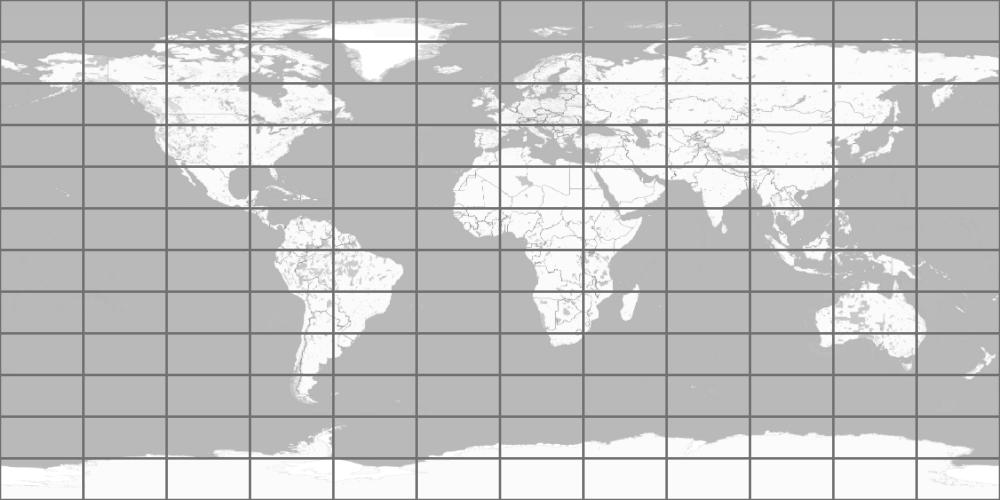
\includegraphics[width=0.9\tw]{projection-platecarree.jpg}
        \caption{Плоская прямоугольная проекция}
        \label{pic:map-projection-plate-carree}
    \end{subcaptionblock}
    \hfill
    \begin{subcaptionblock}[b]{0.49\tw}
        \centering
        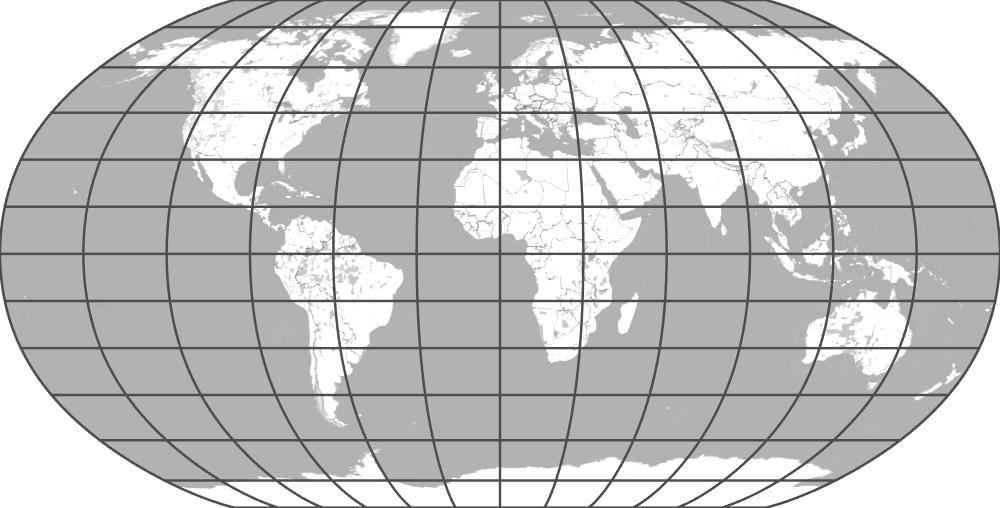
\includegraphics[width=0.9\tw]{projection-robinson.jpg}
        \caption{Проекция Робинсона}
        \label{pic:map-projection-plate-robinson}
    \end{subcaptionblock}
    \\
    \begin{subcaptionblock}[b]{0.49\tw}
        \centering
        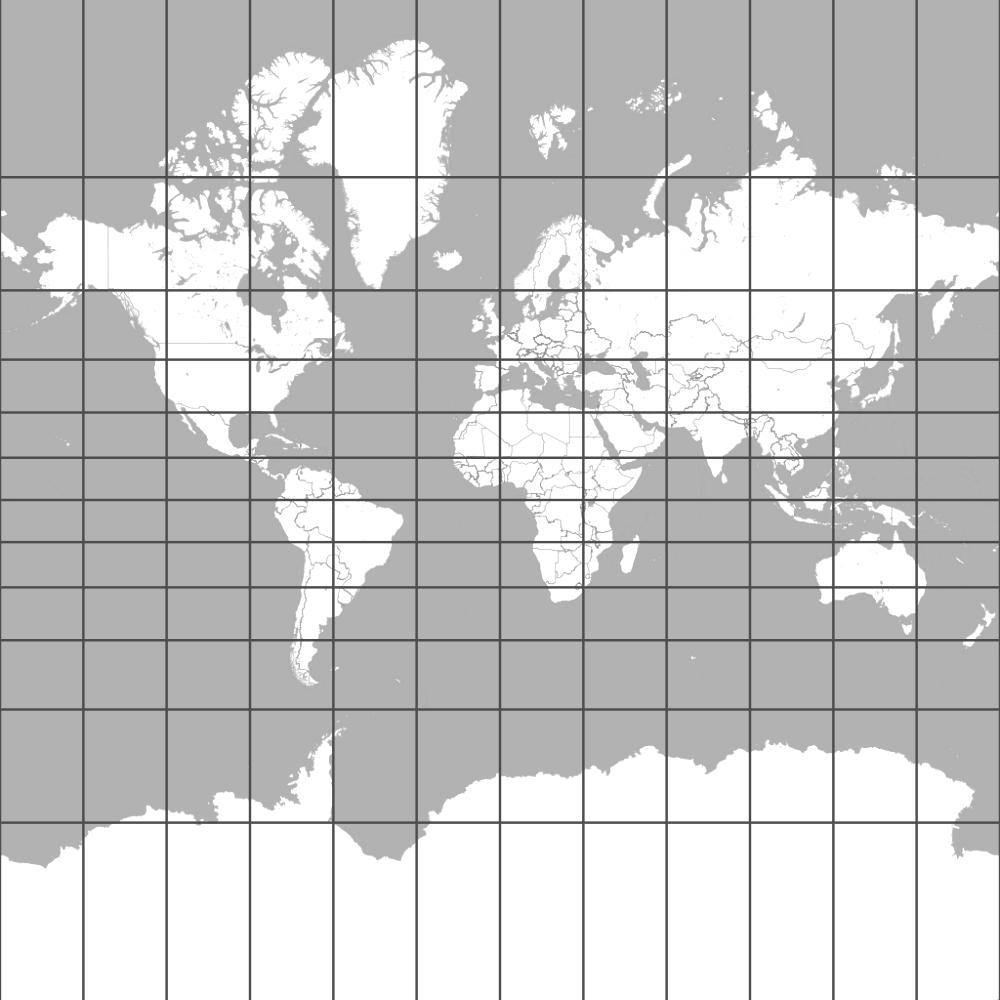
\includegraphics[width=0.9\tw]{projection-mercator.jpg}
        \caption{Проекция Меркатора}
        \label{pic:map-projection-mercator}
    \end{subcaptionblock}
    \hfill
    \begin{subcaptionblock}[b]{0.49\tw}
        \centering
        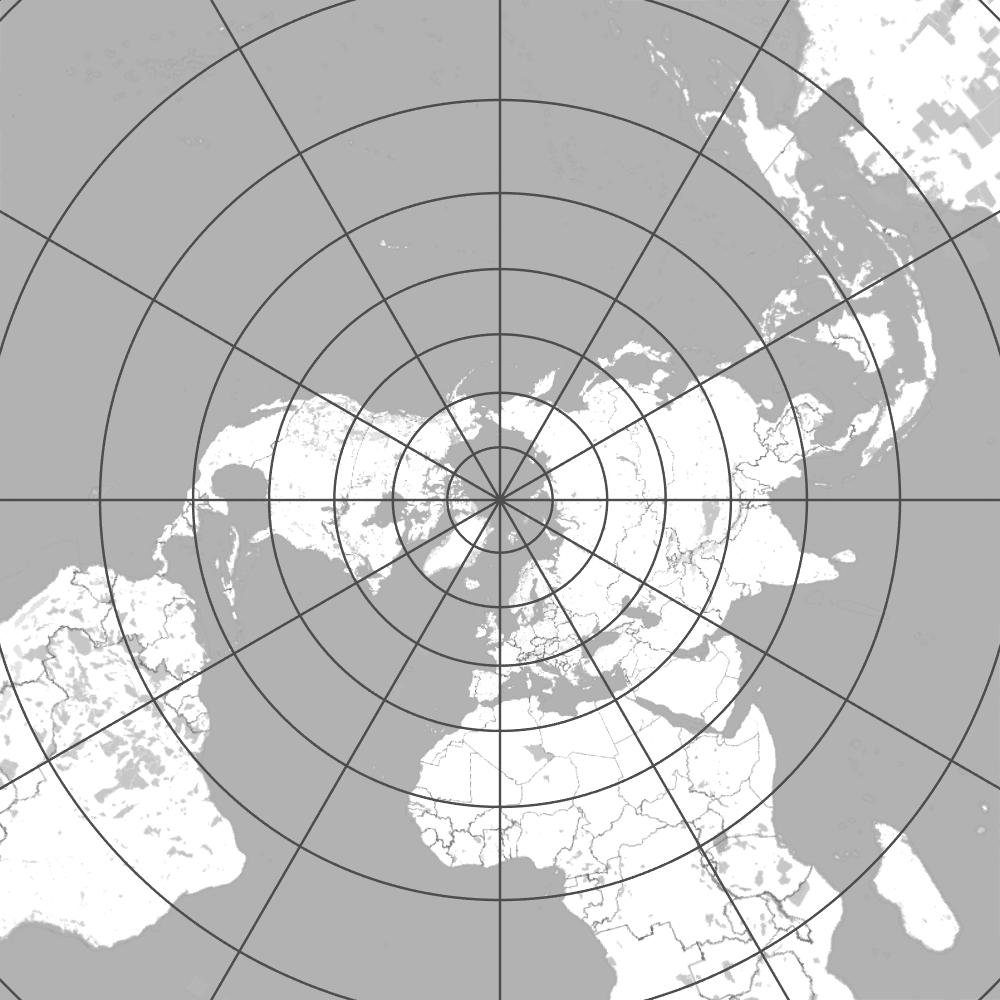
\includegraphics[width=0.9\tw]{projection-stereographic.jpg}
        \caption{Стереографическая проекция}
        \label{pic:map-projection-stereographic}
    \end{subcaptionblock}
    \\
    \begin{subcaptionblock}[b]{0.49\tw}
        \centering
        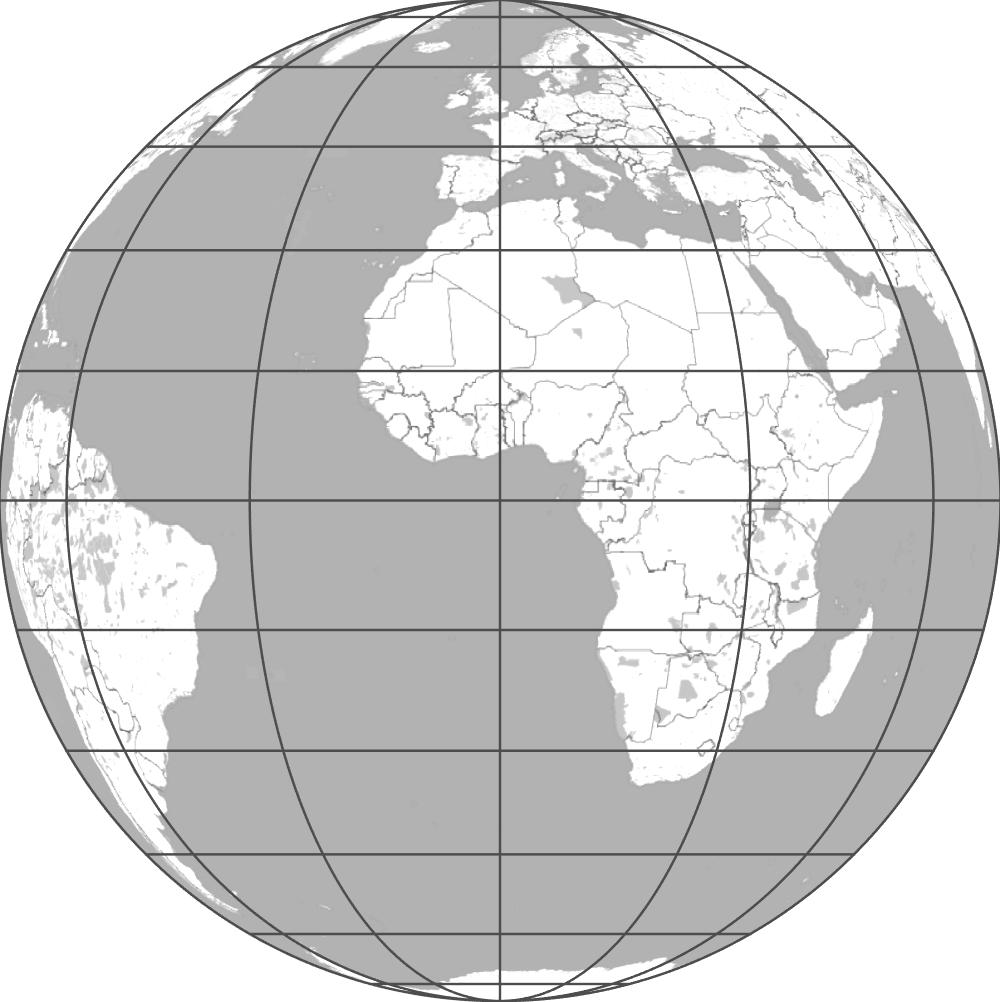
\includegraphics[width=0.9\tw]{projection-orthographic.jpg}
        \caption{Ортографическая проекция}
        \label{pic:map-projection-orthographic}
    \end{subcaptionblock}
    \hfill
    \begin{subcaptionblock}[b]{0.49\tw}
        \centering
        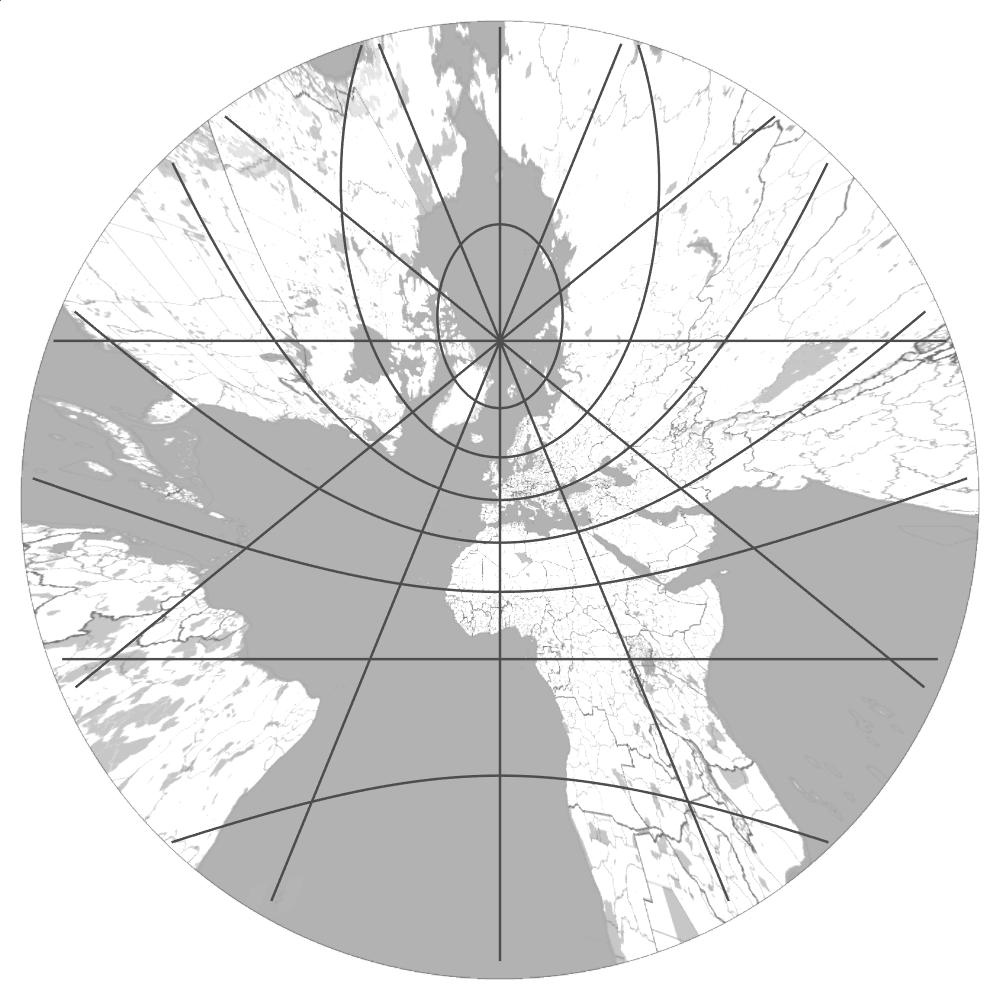
\includegraphics[width=0.9\tw]{projection-gnomonic.jpg}
        \caption{Гномоническая проекция}
        \label{pic:map-projection-gnomonic}
    \end{subcaptionblock}
    \\
    \begin{subcaptionblock}[b]{0.49\tw}
        \centering
        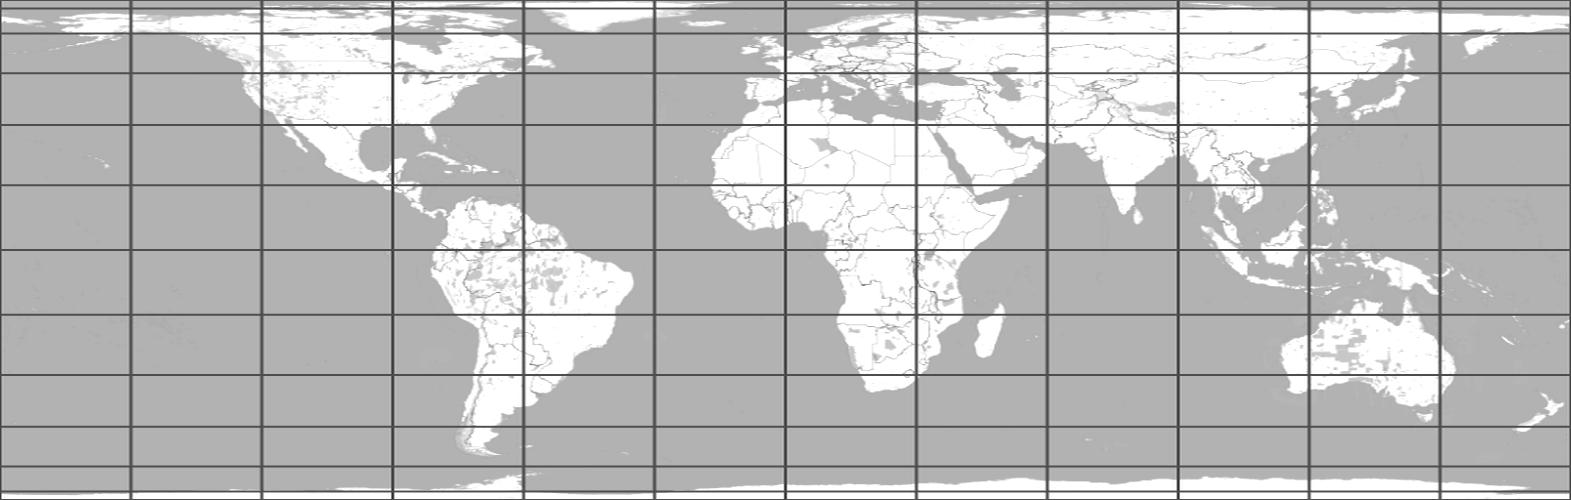
\includegraphics[width=\tw]{projection-lambertcylindrical.jpg}
        \caption{Цилиндрическая проекция Ламберта}
        \label{pic:map-projection-lambertcylindrical}
    \end{subcaptionblock}
    \caption{Картографические проекции}
    \label{pic:map-projection}
\end{figure}
